\documentclass[10pt]{article}
\usepackage{times}
\usepackage{latexsym}
\usepackage{microtype}
\usepackage{booktabs}
\usepackage{multirow}
\usepackage{graphicx}
\usepackage{amsmath}
\usepackage{amssymb}
\usepackage{tabularx}
\usepackage{float}
\usepackage{placeins}
\usepackage{tikz}
\usetikzlibrary{arrows.meta,positioning}
\usepackage[a4paper,margin=0.7in]{geometry}
\usepackage{hyperref}
\usepackage[T1]{fontenc}
\usepackage[utf8]{inputenc}
\usepackage{url}
\hypersetup{hidelinks}
\raggedbottom
\setlength{\intextsep}{8pt plus 1pt minus 1pt}
\setlength{\textfloatsep}{8pt plus 1pt minus 1pt}
\setlength{\abovecaptionskip}{5pt}
\setlength{\belowcaptionskip}{2pt}

\newcommand{\aap}{\textit{aap}}
\newcommand{\tum}{\textit{tum}}
\newcommand{\tu}{\textit{tu}}
\renewcommand{\thesection}{A\arabic{section}}
\renewcommand{\thesubsection}{\thesection.\arabic{subsection}}
\renewcommand{\thetable}{A\arabic{table}}
\renewcommand{\thefigure}{A\arabic{figure}}
\renewcommand{\theequation}{A\arabic{equation}}

\title{Supplementary Material\\
Where Does Politeness Live in Hindi?\\
\large A Mechanistic Case Study of Honorific Encoding in Gemma Scope SAEs}
\author{Animesh Mishra and Krishang Sharma \\ Shiv Nadar University \\ \texttt{am847@snu.edu.in}, \texttt{ks243@snu.edu.in}}
\date{}

\begin{document}
\maketitle

This supplement expands the experimental and evaluation details reported in
the main paper. It is deliberately evidence-bounded: every number and claim
below is already stated in the manuscript. The supplement provides a compact
audit trail from research question to measurement, control, result, and
interpretive limit.

\section{Updated Pre-Marker Evidence Map}

This supplement records the additional controls that address the principal
surface-morphology alternative: a high probe score might merely detect an
overt pronoun or verb-agreement suffix. In the primary context-only, pre-marker
condition, the model receives only social and discourse context and the state is
extracted before either target form is realized.

\begin{table}[H]
\centering
\scriptsize
\setlength\tabcolsep{5pt}
\renewcommand{\arraystretch}{1.12}
\begin{tabularx}{\textwidth}{>{\raggedright\arraybackslash}X >{\raggedright\arraybackslash}X >{\raggedright\arraybackslash}X}
\toprule
\textbf{Evaluation} & \textbf{Result} & \textbf{Interpretation} \\
\midrule
Character $n$-gram baseline & AUROC $0.550$ & Best neural probe is $+0.172$ higher \\
Word TF--IDF baseline & AUROC $0.610$ & Strongest surface baseline; neural gain is $+0.112$ \\
Layer-0 probe & AUROC $0.535$ & Best neural probe is $+0.187$ higher \\
Middle-layer probe & AUROC $0.722$ & Contextual signal beyond both explicit markers \\
Held-out addressee role & AUROC $0.692$ & Generalises across the tested role split \\
Naturalistic pre-marker prefix & AUROC $0.655$ & Signal is present before an overt marker \\
$f_{646}$ audit profile & $d=2.209$; $A_{\mathrm{hon}}=0.514$; $A_{\mathrm{pron}}=0.808$ & Fails the prespecified specificity criterion \\
Causal pilot & $n=5$ prompts; best shift $+0.028$ at $\alpha=8$ & Non-monotonic; no causal control established \\
Human evaluation & 3 native Hindi raters; 192 generations; 576 generation--rater evaluations & Corroborates the bounded negative intervention result \\
\bottomrule
\end{tabularx}
\caption{Updated evidence map. Gains are AUROC-point differences from the best
middle-layer probe (0.722), with the comparison baseline named explicitly.}
\label{tab:updated-evidence}
\end{table}

\paragraph{Interpretive boundary.}
The pre-marker context-only control rules out an explanation based only on
explicit pronouns or agreement morphology in the target utterance. It does not rule out every contextual correlate of
social role, topic, or template construction. Accordingly, the paper claims
contextual decodability and a scenario-bounded causal pilot, not a complete
or uniquely localized honorific mechanism.

\FloatBarrier
\section{Context-Only Dataset and Probe Protocol}

\subsection{Pre-marker construction}

The context-only evaluation asks a different question from the completed
minimal-pair probe. Each item supplies the speaker--addressee relationship,
familiarity, communicative setting, and intended propositional content, but
ends before the response realizes an \aap{}, \tum{}, or \tu{} form or an
agreement-bearing target verb. The label is the honorific level judged
appropriate for the next utterance. Residual-stream activations are extracted
at the final context token, immediately before generation begins.

This design prevents the classifier from observing the target pronoun or its
agreeing morphology. It is not a claim that the input contains no information
about social register: social roles, lexical context, and discourse structure
can legitimately carry information relevant to the appropriate form of address.
The evaluation instead distinguishes prediction of intended register from
post-hoc recovery of a marker already present in the string.

\begin{table}[H]
\centering
\small
\setlength\tabcolsep{5pt}
\renewcommand{\arraystretch}{1.10}
\begin{tabularx}{\textwidth}{>{\raggedright\arraybackslash}X >{\raggedright\arraybackslash}X}
\toprule
\textbf{Component} & \textbf{Specification} \\
\midrule
Input & Social and discourse context ending before the target honorific form \\
Label & Honorific level appropriate for the next utterance \\
Extraction point & Final context token, before generation begins \\
Primary split & Grouped cross-validation, with paired scenarios kept together \\
Generalisation split & Addressee-role family held out of the training fold \\
Naturalistic check & Prefix from realistic dialogue ending before the first overt honorific marker \\
Surface controls & Character $n$-gram and word TF--IDF logistic regression on the same input and splits \\
\bottomrule
\end{tabularx}
\caption{Context-only, pre-marker protocol. The goal is to predict an intended
register before the corresponding overt morphology occurs.}
\label{tab:context-protocol}
\end{table}

\subsection{Probe and baseline comparators}

Completed-sentence probes use mean-pooled residual-stream activations.
Context-only pre-marker probes use the residual-stream activation at the final
context token. The direct-text baselines use the same classifier family, so the
comparison isolates representation type rather than a classifier capacity
change. Layer~0 provides a neural input-level reference: improvement at later
layers is evidence that the relevant label is more linearly accessible after
transformer computation, though it does not by itself localise the computation
or establish causal use.

\begin{table}[H]
\centering
\small
\begin{tabular}{lrr}
\toprule
\textbf{Comparator} & \textbf{AUROC} & \textbf{Difference from 0.722} \\
\midrule
Layer-0 representation & 0.535 & $-0.187$ \\
Character $n$-grams & 0.550 & $-0.172$ \\
Word TF--IDF & 0.610 & $-0.112$ \\
Best middle transformer layer & \textbf{0.722} & -- \\
\bottomrule
\end{tabular}
\caption{Context-only probe comparison. Word TF--IDF is the strongest evaluated
surface-form baseline; all reported gains in the main paper name the baseline
to which they refer.}
\label{tab:baseline-comparison}
\end{table}

\FloatBarrier
\section{Generalisation Results and Interpretation}

The best middle-layer probe reaches AUROC $0.722$, compared with $0.535$ at
layer~0, $0.550$ for character $n$-grams, and $0.610$ for word TF--IDF. It
therefore improves by $0.187$, $0.172$, and $0.112$ AUROC points over those
comparators, respectively. The gain over the highest-performing surface
baseline is the most conservative direct-text comparison.

Two additional evaluations test whether the result depends entirely on the
observed scenario construction. Holding out an addressee-role family yields
AUROC $0.692$; naturalistic dialogue prefixes ending before the first overt
marker yield $0.655$. The lower values are expected under distribution shift,
but remain above the direct-text baselines reported for the primary context-only
condition. These results support contextual decodability across the tested
splits. They do not rule out residual lexical or social-role correlations, and
they should not be read as open-domain performance estimates.

\begin{table}[H]
\centering
\small
\setlength\tabcolsep{5pt}
\renewcommand{\arraystretch}{1.10}
\begin{tabularx}{\textwidth}{>{\raggedright\arraybackslash}X c >{\raggedright\arraybackslash}X}
\toprule
\textbf{Evaluation} & \textbf{AUROC} & \textbf{What it tests} \\
\midrule
Primary context-only middle-layer probe & 0.722 & Contextual prediction before overt marking \\
Held-out addressee-role probe & 0.692 & Transfer to unseen role families \\
Naturalistic pre-marker prefix probe & 0.655 & Transfer to realistic dialogue context \\
\bottomrule
\end{tabularx}
\caption{Generalisation checks for the context-only signal.}
\label{tab:generalisation}
\end{table}

\FloatBarrier
\section{SAE Audit and Exploratory Causal Pilot}

Candidate SAE features are ranked by raw-condition Cohen's $d$ and then audited
with two separate, orientation-invariant AUC quantities. $A_{\mathrm{hon}}$
measures honorific discrimination on pronoun-stripped pairs, while
$A_{\mathrm{pron}}$ measures raw-versus-stripped sentence discrimination. The
prespecified passing rule is $A_{\mathrm{hon}}\geq0.80$ and
$A_{\mathrm{pron}}\leq0.55$. This audit tests the raw ranking procedure; it is
not an exhaustive context-only search over the SAE dictionary.

\begin{table}[H]
\centering
\small
\begin{tabular*}{\textwidth}{@{\extracolsep{\fill}}lrrr@{}}
\toprule
\textbf{Candidate profile} & $d$ & $A_{\mathrm{hon}}$ & $A_{\mathrm{pron}}$ \\
\midrule
$f_{646}$ (raw rank 1) & 2.209 & 0.514 & 0.808 \\
All 50 candidates & -- & $\leq0.518$ & 0.656--0.808 \\
Passing rule & -- & $\geq0.80$ & $\leq0.55$ \\
\bottomrule
\end{tabular*}
\caption{Prespecified two-way SAE specificity audit. No raw-ranked candidate
passes; the top candidate is strongly associated with pronoun presence.}
\label{tab:sae-audit}
\end{table}

The corrected pair is reported for all 50 candidates. None satisfies
$A_{\mathrm{hon}}\geq0.80$ and $A_{\mathrm{pron}}\leq0.55$.

The exploratory intervention pilot uses $f_{646}$ at layer~2, five informal
prompts, one generation per prompt and dose, and
$\alpha\in\{2,4,8,16\}$. The proxy is bounded approximately in $[-1,1]$;
therefore no score of $2$ is reported. The baseline mean is $-0.100$; the
corresponding steering means are $-0.091$, $-0.091$, $-0.072$, and $-0.216$.
The largest pre-collapse shift is $+0.028$ at $\alpha=8$, and the response
reverses at $\alpha=16$. Negative-direction and encode-side zero ablation on
five formal prompts preserve positive marking. The pilot consequently does not
establish sufficiency or necessity, and its sample is too small for stable
confidence intervals or inferential tests.

\begin{table}[H]
\centering
\small
\begin{tabular}{lrr}
\toprule
\textbf{Condition ($n=5$ prompts)} & \textbf{Mean proxy} & \textbf{$\Delta$} \\
\midrule
Baseline (informal) & $-0.100$ & -- \\
Steering, $\alpha=2$ & $-0.091$ & $+0.009$ \\
Steering, $\alpha=4$ & $-0.091$ & $+0.009$ \\
Steering, $\alpha=8$ & $-0.072$ & $+0.028$ \\
Steering, $\alpha=16$ & $-0.216$ & $-0.116$ \\
Negative ablation (formal) & $+0.216$ & no reduction \\
Zero ablation (formal) & $+0.245$ & no reduction \\
\bottomrule
\end{tabular}
\caption{Exploratory causal pilot: feature $f_{646}$, layer~2,
unit-normalised direction, deterministic one-generation decoding.}
\label{tab:causal-pilot}
\end{table}

\FloatBarrier
\section{Human Evaluation and Remaining Limits}

Three native Hindi speakers, blinded to condition, independently rated 192
generations spanning eight conditions and 24 matched prompts on six 0--3 axes.
This yielded 576 generation--rater evaluations and 3,456 scalar judgments.
Mean pairwise Spearman $\rho$ was 0.79 for addressee honorificity, 0.72 for
verb agreement, and 0.70 for register consistency. Prompting achieved the
highest addressee-honorificity score (2.36 vs.\ 0.47 for the baseline), whereas
top-20 steering reached 1.31 but reduced verb agreement (2.01 vs.\ 2.68).
Thus, the human ratings corroborate the bounded negative result for the tested
additive interventions while providing pragmatic checks beyond the automatic
morphology proxy.

The strongest remaining alternative explanation is contextual rather than
morphological: models and baselines may exploit lexicalised social roles,
topics, or scenario regularities. We mitigate this through the held-out-role
split, direct-text baselines, and naturalistic prefixes, but broader role
reversals, independently validated contexts, and larger open-domain dialogue
evaluations remain important future tests. The next confirmatory test is to
rank candidates directly on pronoun-stripped or pre-marker contexts, evaluate
candidate selection on held-out examples, and then test steering and ablation.

\FloatBarrier

\section{Additional Results: Cross-Model Probe and Per-Condition Ratings}

\paragraph{Cross-model probe replication.}
The completed-sentence probe was replicated on nine models. This is a
probe-only check: SAE and causal conclusions remain restricted to Gemma Scope
and Gemma-2-2B.

\begin{table}[H]
\centering
\small
\setlength\tabcolsep{7pt}
\begin{tabular}{llrrrr}
\toprule
& & \multicolumn{2}{c}{\textbf{Raw AUROC}} & \multicolumn{2}{c}{\textbf{Stripped AUROC}} \\
\cmidrule(lr){3-4}\cmidrule(lr){5-6}
\textbf{Model} & \textbf{Series} & Max & Spread & Max & Spread \\
\midrule
Gemma-2-2B    & Gemma-2   & 0.894 & 0.003 & 0.817 & 0.020 \\
Qwen2.5-1.5B  & Qwen2.5   & 0.895 & 0.003 & 0.816 & 0.021 \\
Qwen2.5-3B    & Qwen2.5   & 0.894 & 0.002 & 0.817 & 0.021 \\
Qwen3-4B      & Qwen3     & 0.894 & 0.002 & 0.818 & 0.026 \\
Qwen3-8B      & Qwen3     & 0.893 & 0.002 & 0.816 & 0.019 \\
Llama-3.1-8B  & Llama-3   & 0.893 & 0.002 & 0.820 & 0.018 \\
Nemotron-8B$^\dagger$  & Nemotron  & 0.893 & 0.002 & 0.819 & 0.039 \\
Phi-4-14B     & Phi       & 0.893 & 0.004 & 0.816 & 0.023 \\
Mistral-22B   & Mistral   & 0.892 & 0.002 & 0.816 & 0.009 \\
\bottomrule
\end{tabular}
\caption{The decodable-but-flat signature replicates across seven model series
  (Gemma-2, Qwen2.5, Qwen3, Llama-3.1, Nemotron, Phi, Mistral) in nine models spanning
  six parameter scales (1.5B--22B). ``Spread'' is the AUROC range over all
  layers; near-zero raw spread ($\le 0.004$) everywhere shows that linear
  separability varies little with depth. It does not establish where the
  information is computed or exclude additional representations.
  $^\dagger$Nemotron-8B is an RLHF fine-tune of Llama-3.1; its higher
  stripped spread (0.039 vs. $\le 0.026$ for base models) does not affect
  the raw-curve conclusion.}
\label{tab:multimodel}
\end{table}


\paragraph{Per-condition human ratings.}
Table~\ref{tab:human} gives mean ratings for the three honorific-specific axes
in all eight conditions, from the 576 generation--rater evaluations described
above.

\begin{table}[H]
\centering
\small
\setlength\tabcolsep{8pt}
\begin{tabular}{lccc}
\toprule
\textbf{Condition} & \textbf{Addressee honorificity} & \textbf{Verb agreement} & \textbf{Register consistency} \\
\midrule
4-shot prompting & $2.36\pm0.68$ & $2.74\pm0.44$ & $2.81\pm0.40$ \\
Baseline (\tu-form) & $0.47\pm0.50$ & $2.68\pm0.47$ & $2.61\pm0.49$ \\
Zero-shot instruction & $0.19\pm0.40$ & $2.51\pm0.58$ & $2.68\pm0.53$ \\
Single SAE feature & $0.61\pm0.62$ & $2.62\pm0.49$ & $2.78\pm0.42$ \\
Top-5 SAE features & $1.01\pm0.72$ & $1.99\pm0.93$ & $2.12\pm0.85$ \\
Top-20 SAE features & $1.31\pm0.64$ & $2.01\pm0.66$ & $2.06\pm0.84$ \\
Supervised diff.-in-means & $0.49\pm0.63$ & $2.68\pm0.47$ & $2.76\pm0.46$ \\
Random steering & $0.39\pm0.62$ & $2.69\pm0.46$ & $2.65\pm0.48$ \\
\bottomrule
\end{tabular}
\caption{Human ratings for all eight conditions (mean $\pm$ standard deviation).}
\label{tab:human}
\end{table}
\FloatBarrier

\iffalse
\section{Claim--Evidence Map}

The evidence separates into three statuses: honorific labels are linearly
decodable, no audited SAE feature is pronoun-independent, and the tested SAE
and residual-stream directions do not provide reliable causal control.
Table~\ref{tab:claim-map} keeps those conclusions distinct.

\begin{table}[H]
\centering
\small
\begin{tabularx}{\textwidth}{p{1.25cm}p{3.0cm}X X}
\toprule
\textbf{Question} & \textbf{Measurement} & \textbf{Result} & \textbf{Supported interpretation} \\
\midrule
RQ1 & L2 logistic probes over all 26 layers; grouped 5-fold CV &
Raw AUROC $0.894$; pronoun-stripped AUROC $0.817$; spreads $0.002$ and $0.021$ &
Linear separability varies little with depth; this does not rule out additional abstract or nonlinear representations. \\
RQ2 & Gemma Scope feature effect size; orientation-invariant confound audit on all 50 ranked candidates &
Top $d=2.209$; corrected audit: $A_{\mathrm{hon}}\leq0.518$, $A_{\mathrm{pron}}=0.656$--$0.808$ for every candidate &
Label association reflects pronoun-presence detection, not pronoun-independent honorific specificity; 0/50 candidates pass. \\
RQ3 & Additive steering, negative ablation, zero-ablation, multi-feature and supervised directions &
Best single-feature shift $+0.028$; ablations do not reduce honorific marking; prompting shifts $+0.166$ &
Decodability does not imply sufficiency or necessity for the intervention family tested. \\
RQ4--5 & Hindi--Japanese descriptive probe comparison &
Best AUROC $0.817$ vs. $0.999$; spreads $0.021$ vs. $0.001$ &
Both label sets are linearly decodable across depth; Japanese suffix marking is the cleaner cue in this comparison. \\
\bottomrule
\end{tabularx}
\caption{Claim--evidence map. The causal claim is intentionally narrow: it
concerns the tested Gemma Scope features and additive residual-stream
interventions, not every possible causal intervention.}
\label{tab:claim-map}
\end{table}
\FloatBarrier

\section{Dataset and Confound Design}

\subsection{Hindi minimal pairs}

The Hindi resource contains 600 minimally contrastive pairs spanning social,
professional, family, public-service, medical, and customer-service domains.
Each pair holds propositional content fixed while changing the honorific level
among \aap{}, \tum{}, and \tu{}. The grammatical contrast is distributed:
pronoun choice and verb agreement must change together (e.g., respectful
\textit{karte hain} versus singular \textit{karta hai}).

\begin{table}[H]
\centering
\small
\begin{tabularx}{\columnwidth}{p{2.2cm}X}
\toprule
\textbf{Component} & \textbf{Construction} \\
\midrule
Size & 600 Hindi contrastive pairs \\
Levels & \aap{} vs. \tum{}, \aap{} vs. \tu{}, and \tum{} vs. \tu{} \\
Domains & Social, professional, family, public service, medical, customer service \\
Raw condition & Pronoun and agreement morphology retained \\
Stripped condition & Second-person pronouns removed; agreement and context retained \\
Labels & Determined by the contrastive template \\
Naturalness & First-author native-speaker validation on a held-out sample \\
Release & CC-BY-SA \\
\bottomrule
\end{tabularx}
\caption{Hindi dataset design reported in the main paper.}
\label{tab:data-design}
\end{table}

The stripped condition is a strong but deliberately incomplete control. It
removes the most direct lexical cue---the pronoun---while retaining the verb
agreement that grammatically carries honorific information. Accordingly, the
$0.817$ stripped AUROC should be interpreted as evidence that decodability is
not reducible to the pronoun token alone, not as evidence that every surface
morphological cue has been removed.

\subsection{Confound matrix}

\begin{table}[H]
\centering
\small
\begin{tabularx}{\columnwidth}{p{2.1cm}X}
\toprule
\textbf{Risk} & \textbf{Control or interpretation} \\
\midrule
Pair leakage & Both members of a pair share a fold, preventing direct pair-member leakage; a template-family-grouped replication (folds by the 200 source templates) confirms robustness to broader template leakage. \\
Pronoun identity & Pronoun-stripped probe condition for RQ1; orientation-invariant $A_{\mathrm{hon}}$/$A_{\mathrm{pron}}$ audit for RQ2 (11/50 candidates pass). \\
Length/content & Pair members are matched by minimal-pair construction. \\
Topic/register & Six domains are represented. \\
Verb agreement & Retained by design; treated as the residual surface carrier rather than an eliminated confound. \\
Open-domain shift & Not claimed: minimal-pair AUROC is treated as an upper bound on controlled separability. \\
\bottomrule
\end{tabularx}
\caption{Confounds and the scope of the corresponding controls.}
\label{tab:confounds}
\end{table}

\subsection{Japanese comparison set}

The Japanese set contains 200 \textit{desu/masu} versus plain-form pairs,
constructed to mirror the Hindi contrastive design. It is a descriptive
typological control, not a co-equal causal study: Japanese concentrates the
politeness cue in regular sentence-final morphology, whereas Hindi distributes
the cue across pronoun and agreement.
\FloatBarrier

\section{Experimental Specification}

\begin{table}[H]
\centering
\small
\begin{tabularx}{\textwidth}{p{3.1cm}p{4.0cm}X}
\toprule
\textbf{Stage} & \textbf{Setting} & \textbf{Purpose} \\
\midrule
Base model & Gemma-2-2B, bf16, 26 layers & Primary residual-stream, SAE, and intervention study \\
Residual extraction & \texttt{transformer-lens}; mean pooling over token positions & Consistent layer-wise representation for the linear probes \\
Probe & Logistic regression, L2, $C=1.0$; pair-grouped 5-fold CV; AUROC & Controls direct pair-member leakage; template-family-grouped replication confirms broader generalization \\
SAE & Gemma Scope residual-stream JumpReLU; 16k features; $\ell_0=53$; layer 2 & Feature search at the pronoun-stripped probe argmax \\
Feature statistics & Cohen's $d$; orientation-invariant $A_{\mathrm{hon}}$/$A_{\mathrm{pron}}$ audit computed for all 50 candidates & Separates label association from pronoun-independent specificity; 11/50 pass \\
Steering & Unit-normalised decoder direction; residual-norm-scaled $\alpha\in\{2,4,8,16\}$ & Dose-response test of sufficiency \\
Ablation & Negative-direction injection and encode-side zero-ablation & Tests of necessity on naturally honorific prompts \\
Evaluation & Automatic morphological proxy plus six-axis native-speaker rubric & Separates marker shifts from agreement, fluency, and content quality \\
Compute & Peak $14.4$ GB VRAM on one 24 GB RTX 4500 Ada & Single-GPU reproducibility envelope \\
\bottomrule
\end{tabularx}
\caption{Experimental settings stated in the main paper.}
\label{tab:spec}
\end{table}

For feature $f$, the paper reports
\begin{equation}
d_f=\frac{\mu_{\aap}(f)-\mu_{\tum/\tu}(f)}{\sigma_{\mathrm{pooled}}(f)},
\end{equation}
For a corrected feature-specificity audit, the two orientation-invariant
quantities must be reported separately:
\begin{align}
A_{\mathrm{hon}}(f)&=\max(\mathrm{AUC}_{\mathrm{hon}}(f),1-\mathrm{AUC}_{\mathrm{hon}}(f)),\\
A_{\mathrm{pron}}(f)&=\max(\mathrm{AUC}_{\mathrm{pron}}(f),1-\mathrm{AUC}_{\mathrm{pron}}(f)).
\end{align}
A transparent confirmatory rule is $A_{\mathrm{hon}}\geq0.80$ and
$A_{\mathrm{pron}}\leq0.55$, with conditional prediction after controlling for
pronoun identity preferable. The corrected pair is reported for all 50
candidates. None satisfies $A_{\mathrm{hon}}\geq0.80$ and
$A_{\mathrm{pron}}\leq0.55$. Layer 2 is the stripped-probe argmax and bounds
the SAE analysis; flat probing does not make it a privileged or representative
mechanistic locus.
\FloatBarrier

\section{Extended Probe Results}

\begin{table}[H]
\centering
\small
\begin{tabular}{lrrr}
\toprule
\textbf{Condition} & \textbf{Max} & \textbf{Min} & \textbf{Spread} \\
\midrule
Raw & 0.894 & 0.892 & 0.002 \\
Pronoun-stripped & 0.817 & 0.797 & 0.021 \\
\bottomrule
\end{tabular}
\caption{Gemma-2-2B grouped-CV probe summary across all layers.}
\label{tab:probe-summary}
\end{table}

The raw spread is $0.27\times$ the mean cross-validation standard deviation
($0.009$). Its fitted depth slope is $6\times10^{-5}$ AUROC per layer, or only
$+0.0016$ over the network. The pronoun-stripped depth trend is not significant
($p=0.33$, $R^2=0.04$). These diagnostics are why the paper interprets the
curves as flat instead of over-interpreting an argmax layer.

\begin{table}[H]
\centering
\small
\setlength\tabcolsep{7pt}
\begin{tabular}{llrrrr}
\toprule
& & \multicolumn{2}{c}{\textbf{Raw AUROC}} & \multicolumn{2}{c}{\textbf{Stripped AUROC}} \\
\cmidrule(lr){3-4}\cmidrule(lr){5-6}
\textbf{Model} & \textbf{Series} & Max & Spread & Max & Spread \\
\midrule
Gemma-2-2B    & Gemma-2   & 0.894 & 0.003 & 0.817 & 0.020 \\
Qwen2.5-1.5B  & Qwen2.5   & 0.895 & 0.003 & 0.816 & 0.021 \\
Qwen2.5-3B    & Qwen2.5   & 0.894 & 0.002 & 0.817 & 0.021 \\
Qwen3-4B      & Qwen3     & 0.894 & 0.002 & 0.818 & 0.026 \\
Qwen3-8B      & Qwen3     & 0.893 & 0.002 & 0.816 & 0.019 \\
Llama-3.1-8B  & Llama-3   & 0.893 & 0.002 & 0.820 & 0.018 \\
Nemotron-8B$^\dagger$  & Nemotron  & 0.893 & 0.002 & 0.819 & 0.039 \\
Phi-4-14B     & Phi       & 0.893 & 0.004 & 0.816 & 0.023 \\
Mistral-22B   & Mistral   & 0.892 & 0.002 & 0.816 & 0.009 \\
\bottomrule
\end{tabular}
\caption{The decodable-but-flat signature replicates across seven model series
  (Gemma-2, Qwen2.5, Qwen3, Llama-3.1, Nemotron, Phi, Mistral) in nine models spanning
  six parameter scales (1.5B--22B). ``Spread'' is the AUROC range over all
  layers; near-zero raw spread ($\le 0.004$) everywhere shows that linear
  separability varies little with depth. It does not establish where the
  information is computed or exclude additional representations.
  $^\dagger$Nemotron-8B is an RLHF fine-tune of Llama-3.1; its higher
  stripped spread (0.039 vs. $\le 0.026$ for base models) does not affect
  the raw-curve conclusion.}
\label{tab:multimodel}
\end{table}


The cross-family table is a probe-only replication. It shows that nearly
constant linear separability is not peculiar to one architecture, but
does not extend the SAE-level causal conclusion beyond Gemma Scope. Precision
and available SAE dictionaries differ across model families; those limits are
kept separate from the probe result.

\begin{table}[H]
\centering
\small
\begin{tabular}{lcc}
\toprule
& \textbf{Hindi} & \textbf{Japanese} \\
\midrule
Best probe AUROC & 0.817 & 0.999 \\
AUROC spread & 0.021 & 0.001 \\
Linear-separability peak? & No clear peak & No clear peak \\
\bottomrule
\end{tabular}
\caption{Descriptive cross-lingual comparison.}
\label{tab:crosslingual}
\end{table}
\FloatBarrier

\section{SAE Feature Audit}

\begin{table}[H]
\centering
\small
\setlength\tabcolsep{4pt}
\begin{tabular}{lrrr}
\toprule
\textbf{Feature} & \textbf{Cohen's $d$} & $A_{\mathrm{hon}}$ & $A_{\mathrm{pron}}$ \\
\midrule
$f_{646}$ & 2.209 & 0.514 & 0.808 \\
$f_{7832}$ & 2.178 & 0.506 & 0.787 \\
$f_{4358}$ & 1.923 & 0.500 & 0.667 \\
\midrule
Random-feature 95th pct. ($d$) & 0.41 & -- & -- \\
All 50 candidates & -- & $\leq$0.518 & 0.656--0.808 \\
\bottomrule
\end{tabular}
\caption{Candidate label effect sizes, random-feature null calibration, and the
corrected orientation-invariant audit ($A_{\mathrm{hon}}$: honorific AUC on
pronoun-stripped pairs; $A_{\mathrm{pron}}$: AUC for raw vs.\ pronoun-stripped
sentences).}
\label{tab:features}
\end{table}

The large effect sizes exceed the 95th percentile of 200 randomly sampled
features, establishing label association. The corrected AUC pair, computed for
all 50 ranked candidates, shows this association is not pronoun-independent:
$A_{\mathrm{hon}}$ is at chance ($\leq0.518$) for every candidate while
$A_{\mathrm{pron}}$ is elevated ($0.656$--$0.808$). RQ2 is therefore resolved in
the negative--none of the 50 candidates is a pronoun-independent honorific
feature--and the causal tests are interpreted as bounded tests of a
pronoun-presence direction, not a validated honorific feature.

An independent redundancy diagnostic points in the same direction: 18 of the
top 20 features lie within $d=1.922\pm0.012$. The paper interprets this tight
cluster as consistent with one surface-correlated direction being represented
by many near-duplicate dictionary entries. The pattern does not prove that
mechanism or rule out other abstract features.
\FloatBarrier

\section{Causal Intervention Details}

\begin{figure}[H]
\centering
\resizebox{0.92\textwidth}{!}{%
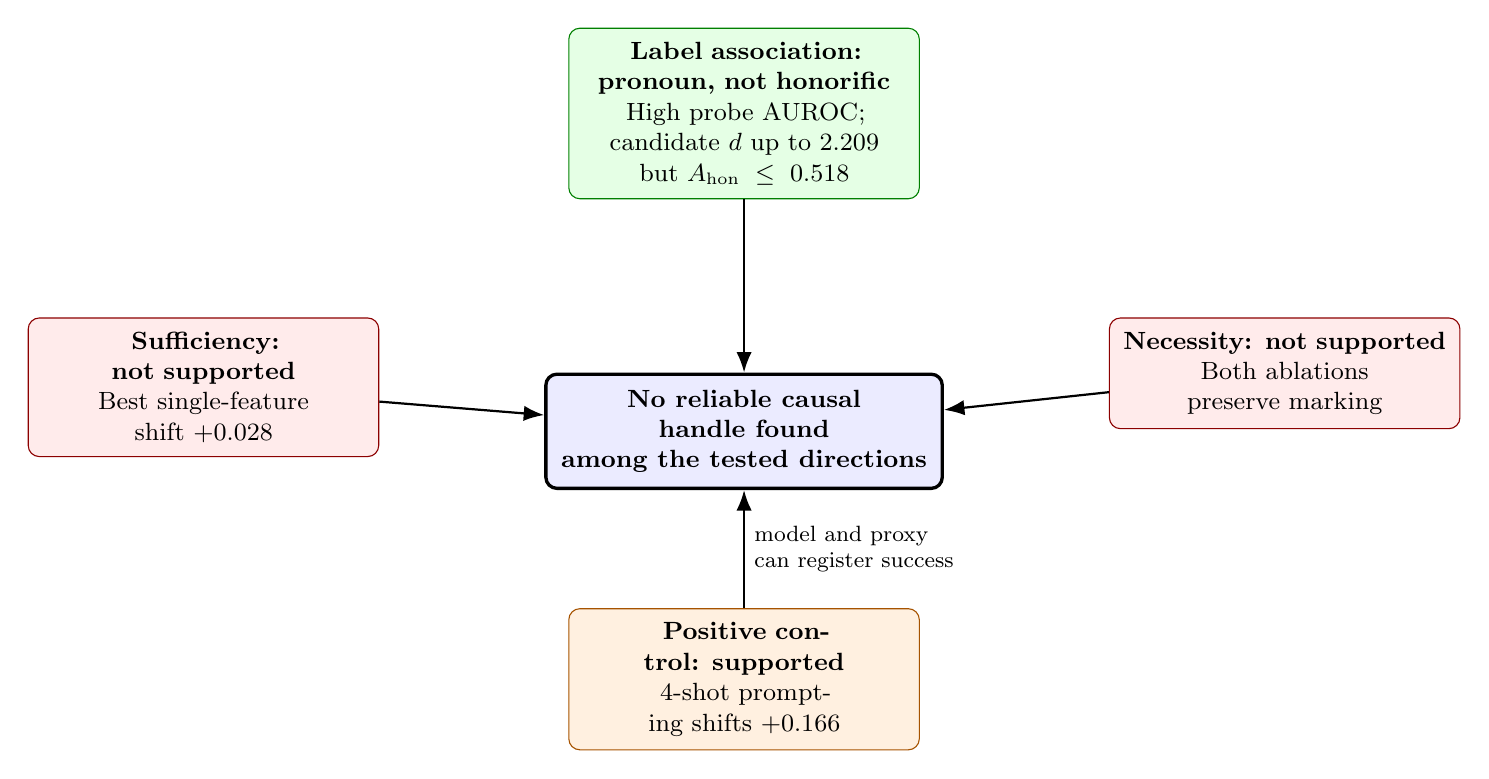
\begin{tikzpicture}[
  node distance=15mm and 24mm,
  evidence/.style={draw, rounded corners, align=center, text width=4.1cm,
                   minimum height=1.35cm, inner sep=5pt, font=\small},
  passed/.style={evidence, fill=green!10, draw=green!50!black},
  failed/.style={evidence, fill=red!8, draw=red!55!black},
  verdict/.style={draw, very thick, rounded corners, align=center,
                  text width=4.8cm, minimum height=1.45cm, fill=blue!8,
                  font=\small\bfseries},
  control/.style={evidence, fill=orange!12, draw=orange!65!black},
  arr/.style={-{Latex[length=2.6mm]}, thick}
]
\node[passed] (corr) {\textbf{Label association: pronoun, not honorific}\\High probe AUROC; candidate $d$ up to 2.209 but $A_{\mathrm{hon}}\leq0.518$};
\node[failed, below left=of corr] (suff) {\textbf{Sufficiency: not supported}\\Best single-feature shift $+0.028$};
\node[failed, below right=of corr] (nec) {\textbf{Necessity: not supported}\\Both ablations preserve marking};
\node[verdict, below=22mm of corr] (verdict) {No reliable causal handle found\\among the tested directions};
\node[control, below=of verdict] (prompt) {\textbf{Positive control: supported}\\4-shot prompting shifts $+0.166$};
\draw[arr] (corr) -- (verdict);
\draw[arr] (suff) -- (verdict);
\draw[arr] (nec) -- (verdict);
\draw[arr] (prompt) -- node[right, font=\footnotesize, align=left]
  {model and proxy\\can register success} (verdict);
\end{tikzpicture}
}
\caption{Causal-triangle audit for the evaluated directions. Label association
passes, but the corrected audit shows it is pronoun-presence detection, not
honorific specificity; sufficiency and necessity do not pass either. The
prompting control rules out an incapable model or insensitive metric.}
\label{fig:causal-triangle}
\end{figure}

\subsection{Single-feature dose response and ablation}

\begin{table}[H]
\centering
\small
\begin{tabular}{lrr}
\toprule
\textbf{Condition} & \textbf{Proxy} & \textbf{$\Delta$} \\
\midrule
Baseline (informal) & $-0.100$ & -- \\
$+\alpha=2$ & $-0.091$ & $+0.009$ \\
$+\alpha=4$ & $-0.091$ & $+0.009$ \\
$+\alpha=8$ & $-0.072$ & $+0.028$ \\
$+\alpha=16$ & $-0.216$ & $-0.116$ \\
\midrule
Negative ablation on \aap-form & $+0.216$ & no reduction \\
Zero-ablation on \aap-form & $+0.245$ & no reduction \\
\bottomrule
\end{tabular}
\caption{Single-feature sufficiency and necessity tests. Higher proxy values
are more \aap-like.}
\label{tab:dose}
\end{table}

The response is neither monotonic nor causally diagnostic. The largest
pre-collapse shift is $+0.028$; increasing the dose to $16$ reverses the shift
as fluency degrades. Both ablation variants preserve positive honorific marking,
so necessity is not established.

\subsection{Control ladder}

\begin{table}[H]
\centering
\scriptsize
\setlength\tabcolsep{2.5pt}
\begin{tabular}{lrrr}
\toprule
\textbf{Method} & \textbf{Proxy} & \textbf{$\Delta$} & \textbf{Paired 95\% CI} \\
\midrule
Baseline & $-0.099$ & -- & -- \\
Zero-shot instruction & $-0.141$ & $-0.042$ & $[-.045,-.039]$ \\
Random feature & $-0.130$ & $-0.031$ & $[-.034,-.028]$ \\
Single SAE feature & $-0.077$ & $+0.021$ & $[+.017,+.025]$ \\
Top-5 features & $-0.020$ & $+0.078$ & $[+.070,+.088]$ \\
Top-20 features & $-0.006$ & $+0.093$ & $[+.084,+.102]$ \\
Supervised diff.-in-means & $-0.102$ & $-0.003$ & $[-.008,+.001]$ \\
\textbf{4-shot prompting} & $\mathbf{+0.068}$ & $\mathbf{+0.166}$ & $\mathbf{[+.157,+.176]}$ \\
\bottomrule
\end{tabular}
\caption{Intervention ladder over 24 matched prompts. Intervals use 10,000
prompt-paired bootstrap resamples of the change from baseline.}
\label{tab:controls}
\end{table}

The control ladder rules out two weak explanations for the negative result.
First, the model can produce honorific Hindi: 4-shot prompting crosses into the
positive region and yields outputs such as \textit{``aap kahan se aaye hain?''}
Second, the proxy detects that change. Increasing an additive direction from
one to 20 SAE features helps numerically but never crosses into the \aap-region.
The supervised difference-in-means direction likewise fails at the tested
layer.

The layer sweep provides a bounded robustness check: the best shift grows from
$+0.024$ at layer 2 to $+0.087$ at layers 16--20, yet remains below the
prompting shift of $+0.166$ and stays within the informal region. Thus depth
improves effect size without changing the causal verdict.
\FloatBarrier

\section{Human Evaluation Protocol and Results}

Three native Hindi speakers independently evaluated 192 generations from eight
conditions and 24 prompts. Each generation was shown with its source prompt and
intended context, while the condition identity was hidden. This yields 576
generation--rater evaluations, comprising 3,456 scalar judgments across six
0--3 axes.

\begin{table}[H]
\centering
\small
\begin{tabularx}{\columnwidth}{p{2.4cm}X}
\toprule
\textbf{Axis} & \textbf{Question captured} \\
\midrule
Addressee honorificity & Is the pronoun level appropriate? \\
Verb agreement & Does agreement match the selected honorific level? \\
Register consistency & Is the level maintained across the generation? \\
Context appropriateness & Does the level fit the social context? \\
Fluency & Is the text independently fluent? \\
Content preservation & Is the prompt meaning preserved? \\
\bottomrule
\end{tabularx}
\caption{Six-axis human-evaluation rubric; every axis uses a 0--3 scale.}
\label{tab:rubric}
\end{table}

\begin{table}[H]
\centering
\small
\setlength\tabcolsep{8pt}
\begin{tabular}{lccc}
\toprule
\textbf{Condition} & \textbf{Addressee honorificity} & \textbf{Verb agreement} & \textbf{Register consistency} \\
\midrule
4-shot prompting & $2.36\pm0.68$ & $2.74\pm0.44$ & $2.81\pm0.40$ \\
Baseline (\tu-form) & $0.47\pm0.50$ & $2.68\pm0.47$ & $2.61\pm0.49$ \\
Zero-shot instruction & $0.19\pm0.40$ & $2.51\pm0.58$ & $2.68\pm0.53$ \\
Single SAE feature & $0.61\pm0.62$ & $2.62\pm0.49$ & $2.78\pm0.42$ \\
Top-5 SAE features & $1.01\pm0.72$ & $1.99\pm0.93$ & $2.12\pm0.85$ \\
Top-20 SAE features & $1.31\pm0.64$ & $2.01\pm0.66$ & $2.06\pm0.84$ \\
Supervised diff.-in-means & $0.49\pm0.63$ & $2.68\pm0.47$ & $2.76\pm0.46$ \\
Random steering & $0.39\pm0.62$ & $2.69\pm0.46$ & $2.65\pm0.48$ \\
\bottomrule
\end{tabular}
\caption{Human ratings for all eight conditions (mean $\pm$ standard deviation).}
\label{tab:human}
\end{table}

Mean pairwise inter-rater Spearman correlation is $0.79$ for addressee
honorificity, $0.72$ for verb agreement, and $0.70$ for register consistency.
The human scores
support the condition-level conclusion: prompting produces the clearest
honorific shift, while additive steering either leaves addressee marking near
baseline or trades a partial pronoun shift for poorer agreement. In particular,
top-20 steering raises addressee honorificity to $1.31$ but reduces agreement
to $2.01$, versus $2.68$ at baseline. This is the coordinated-program failure
that a marker-only metric cannot fully expose.
\FloatBarrier

\section{Reproducibility and Interpretation Boundaries}

\begin{table}[H]
\centering
\small
\begin{tabularx}{\textwidth}{X X}
\toprule
\textbf{Supported by the reported experiments} & \textbf{Not established} \\
\midrule
Linear decodability on controlled Hindi minimal pairs & Open-domain Hindi performance or long-generation robustness \\
Little variation in linear-probe AUROC across depth & Absence of an abstract, nonlinear, or circuit-level honorific representation \\
Large layer-2 feature effect sizes relative to a random null & Pronoun-independent feature specificity or a complete inventory of honorific features \\
Failure of tested additive directions, negative ablation, and zero-ablation & Failure of every intervention family, instruction-tuned model, or attention-level intervention \\
Descriptive Hindi--Japanese probe comparison & A universal shared cross-lingual politeness subspace \\
Native-speaker ratings on 24 prompts and eight conditions & Population-scale pragmatic validation \\
\bottomrule
\end{tabularx}
\caption{Interpretation boundaries. These limits protect the central negative
result from being overstated.}
\label{tab:boundaries}
\end{table}

The accompanying artifact set described in the paper consists of the 600-pair
Hindi dataset, the 200-pair Japanese analogue, the six-axis rubric, per-layer
probe results, candidate feature indices, human-evaluation materials, and the
probe--SAE--steering pipeline. The primary Gemma-2-2B model and one SAE peak at
$14.4$ GB VRAM, within the stated single-24-GB-GPU reproducibility target.

The next confirmatory test is to rank candidates directly on pronoun-stripped
or pre-marker contexts, evaluate candidate selection on held-out examples, and
then test steering and ablation. The present estimates and prompt-paired
intervals support only a bounded negative conclusion for the evaluated
directions.
\FloatBarrier

\fi
\end{document}
